\chapter{Validazione}\label{chp:validazione}
Poiché i risultati dei modelli analitici sono validi per periodi d'osservazione tendenzialmente infiniti, è stato scelto in fase di validazione di adottare una simulazione di tipo \textit{steady-state}, al fine di inferire statistiche confrontabili con i valori teorici.

Il metodo adottato è stato quello delle batch means con parametri $(b,k) = (256, 64)$ e periodo d'osservazione $\tau = 16384\ min$. La scelta dei parametri è stata effettuata seguendo le linee guida\footnote{Capitolo 8 del libro \textit{"Discrete Event Simulation - A First Course - Lemmis Park"}.}:
\begin{itemize}
\item $b = 256$, rappresenta un buon compromesso fra il mantenimento della variabilità naturale del fenomeno osservato e l'indipendenza tra batch successivi.
\item $k = 64$, al fine di rendere le statistiche campionate indipendenti dalle
condizioni iniziali ed ottenere intervalli di confidenza significativi.
\end{itemize}

Inoltre:
\begin{itemize}
\item Il seed iniziale utilizzato per le simulazioni che seguono in questo capitolo è \texttt{12345}.
\item È stato utilizzato il programma \texttt{estimate} per il calcolo delle realizzazioni degli intervalli di confidenza.
\end{itemize}

\section{Definizione preliminare dei modelli analitici semplificati}
\begin{figure}[ht]
\centering
\begin{subfigure}[b]{0.475\textwidth}  
\centering 
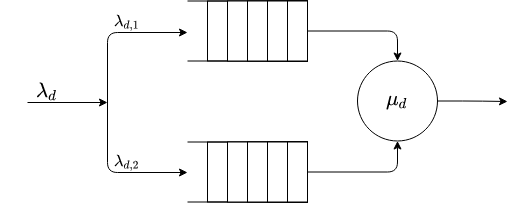
\includegraphics[width=\textwidth]{validazione-modello-analitico-1a}
\caption{Blocco dei ticket \sr{}}    
\label{fig:validazione-modello-analitico-1a}
\end{subfigure}
\hfill 
\begin{subfigure}[b]{0.475\textwidth}
\centering
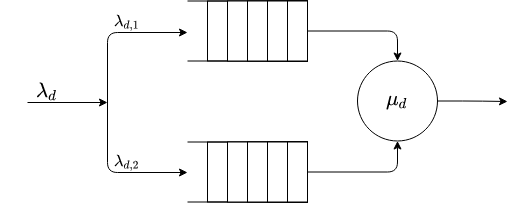
\includegraphics[width=\textwidth]{validazione-modello-analitico-1b}
\caption{Blocco delle altre tipologie di ticket}    
\label{fig:validazione-modello-analitico-1b}
\end{subfigure}
\caption{Modelli analitici semplificati}
\label{fig:validazione-modello-analitico-1}
\end{figure}

Di seguito è riportata un'analisi teorica della rete di Jackson in figura \ref{fig:validazione-modello-analitico-1} necessaria alle sezioni successive della validazione.


\subsection{Descrizione del modello in figura \ref{fig:validazione-modello-analitico-1a}}
Al fine di rendere i risultati teorici confrontabili con quelli della simulazione, si assume che nel modello in figura \ref{fig:validazione-modello-analitico-1a} il servente abbia capacità $M$ volte superiore a quella dei singoli serventi nel multiserver del modello di riferimento.

I parametri di input del sistema \ref{fig:validazione-modello-analitico-1a} sono di seguito riportati:
\begin{itemize}
\item Le probabilità di ricadere in una determinata classe di priorità, sono pari a:
\begin{equation}
\begin{array}{l l}
p_{g,1} = \frac{p_{BP} \cdot p_{UO}}{p_{UO} + p_{PP}} = 0.147059, & p_{g,2} = \frac{p_{BP} \cdot p_{PP}}{p_{UO} + p_{PP}} = 0.102941, \\[1em]
p_{g,3} = \frac{(1-p_{BP}) \cdot p_{UO}}{p_{UO} + p_{PP}} = 0.441176, & p_{g,4} = \frac{(1-p_{BP}) \cdot p_{PP}}{p_{UO} + p_{PP}} = 0.308824, \\[1.5em]
\end{array}
\end{equation}
dove il fattore $\frac{1}{p_{UO} + p_{PP}}$ è necessario per normalizzare le probabilità originali.

\item Definito:
\begin{equation}
\lambda_g = (p_{UO} + p_{PP})\cdot \lambda = 0.207325\ req/min
\end{equation} 

I tassi medi d'arrivo sono pari a:
\begin{equation}
\begin{array}{l l}
\lambda_{g,1} = p_{g,1} \cdot \lambda_g \simeq 0.030489\ req/min, & \lambda_{g,2} = p_{g,2} \cdot \lambda_g \simeq 0.021342\ req/min, \\
\lambda_{g,3} = p_{g,3} \cdot \lambda_g \simeq 0.091467\ req/min, & \lambda_{g,4} = p_{g,4} \cdot \lambda_g \simeq 0.064027\ req/min, \\[1em]
\end{array}
\end{equation}

\item Il tasso di servizio medio è pari a:
\begin{equation}
\label{eqn:validazione-6}
\mu_g = \frac{1}{E[S_g]} = \frac{M}{\frac{14+7}{2}} = \frac{2M}{21}\ req/min
\end{equation}
dove per il calcolo di $E[S_g]$ è stata utilizzata la media dei tempi di servizio delle richieste relative ai ticket \uo{} e \pp{}, assunti in tabella \ref{table:modello-specifiche-1} nel modello delle specifiche.

\item L'occupazione media delle classi $\rho_{g,i} = \lambda_{g,i}/\mu_g$ è pari a:
\begin{equation}
\begin{array}{l l l l}
\rho_{g,1} = \frac{0.320135}{M}, & \rho_{g,2} = \frac{0.224091}{M}, & \rho_{g,3} = \frac{0.960404}{M}, & \rho_{g,4} = \frac{0.672284}{M} \\[1.5em]
\end{array}
\end{equation}
da cui:
\begin{equation}
\label{eqn:validazione-8}
\rho_g = \sum_{i=1}^4 \rho_{g,i} = \frac{2.176914}{M}
\end{equation}
Dalla \ref{eqn:validazione-8} è immediato osservare che è necessario imporre $M \geq 3$ al fine di garantire la stabilità del sistema.
\end{itemize}

Tale sistema è modellato con una coda $M/M/1$ in cui si adotta una disciplina di scheduling astratta. A tal proposito, è possibile utilizzare la KP per calcolare gli indici globali necessari alla validazione, come segue:
\begin{itemize}
\item Il \textbf{tempo medio d'attesa} globale è pari a:
\begin{equation}
\label{eqn:validazione-11}
E[T_{Q_g}]^{KP} = \frac{\rho_g E[S_g]}{1-\rho_g} = \frac{22.8576}{M\cdot (M-2.17691)}\ min
\end{equation}
\item Il \textbf{tempo medio di risposta} globale è pari a:
\begin{equation}
\label{eqn:validazione-13}
E[T_{S_g}] = \frac{1}{\mu_g - \lambda_g} = \frac{10.5}{M-2.17691}\ min
\end{equation}
\end{itemize}

\subsection{Descrizione del modello in figura \ref{fig:validazione-modello-analitico-1b}}

I parametri di input del sistema \ref{fig:validazione-modello-analitico-1b} sono di seguito riportati:
\begin{itemize}
\item Le probabilità di ricadere in una determinata classe di priorità, sono pari a:
\begin{equation}
\begin{array}{l l}
p_{d,1} = \frac{p_{BP} \cdot \cancel{p_{SR}}}{\cancel{p_{SR}}} = 0.25, & p_{d,2} = \frac{(1-p_{BP}) \cdot \cancel{p_{SR}}}{\cancel{p_{SR}}} = 0.75
\end{array}
\end{equation}
dove il fattore $\frac{1}{p_{SR}}$ normalizza le probabilità originali.

\item Definito:
\begin{equation}
\lambda_d = p_{SR}\cdot \lambda = 0.036587\ req/min
\end{equation} 

I tassi medi d'arrivo sono pari a:
\begin{equation}
\begin{array}{l l}
\lambda_{d,1} = p_{d,1} \cdot \lambda_d \simeq 0.009147\ req/min, & \lambda_{d,2} = p_{d,2} \cdot \lambda_d \simeq 0.027440\ req/min
\end{array}
\end{equation}

\item Il tasso di servizio medio è pari a:
\begin{equation}
\mu_d = \frac{1}{E[S_d]} = \frac{1}{10} = 0.1\ req/min
\end{equation}
in accordo alle assunzioni in tabella \ref{table:modello-specifiche-1} nel modello delle specifiche.

\item L'occupazione media delle classi $\rho_{d,j} = \lambda_{d,j}/\mu_d$ è pari a:
\begin{equation}
\begin{array}{l l}
\rho_{d,1} = 0.09147, & \rho_{d,2} = 0.27440
\end{array}
\end{equation}
da cui:
\begin{equation}
\rho_d = \rho_{d,1} + \rho_{d,2} = 0.36587
\end{equation}
\end{itemize}

Tale sistema è modellato con una coda $M/M/1$ in cui si adotta una disciplina di scheduling astratta. A tal proposito, è possibile utilizzare la KP per calcolare gli indici globali necessari alla validazione, come segue:
\begin{itemize}
\item Il \textbf{tempo medio d'attesa} globale, per il sottosistema in figura \ref{fig:validazione-modello-analitico-1b} è pari a:
\begin{equation}
\label{eqn:validazione-24}
E[T_{Q_d}]^{KP} = \frac{\rho_d \cdot E[S_d]}{1-\rho_d} = 5.769637\ min
\end{equation}
\item Il \textbf{tempo medio di risposta} globale, per il sottosistema in figura \ref{fig:validazione-modello-analitico-1b} è pari a:
\begin{equation}
\label{eqn:validazione-26}
E[T_{S_d}] = \frac{1}{\mu_d - \lambda_d} = 15.769637\ min
\end{equation}
\end{itemize}


\section{Blocco del flusso degli arrivi di tipo \sr{}}\label{sec:validazione-blocco-sr}
\begin{figure}[ht]
\centering
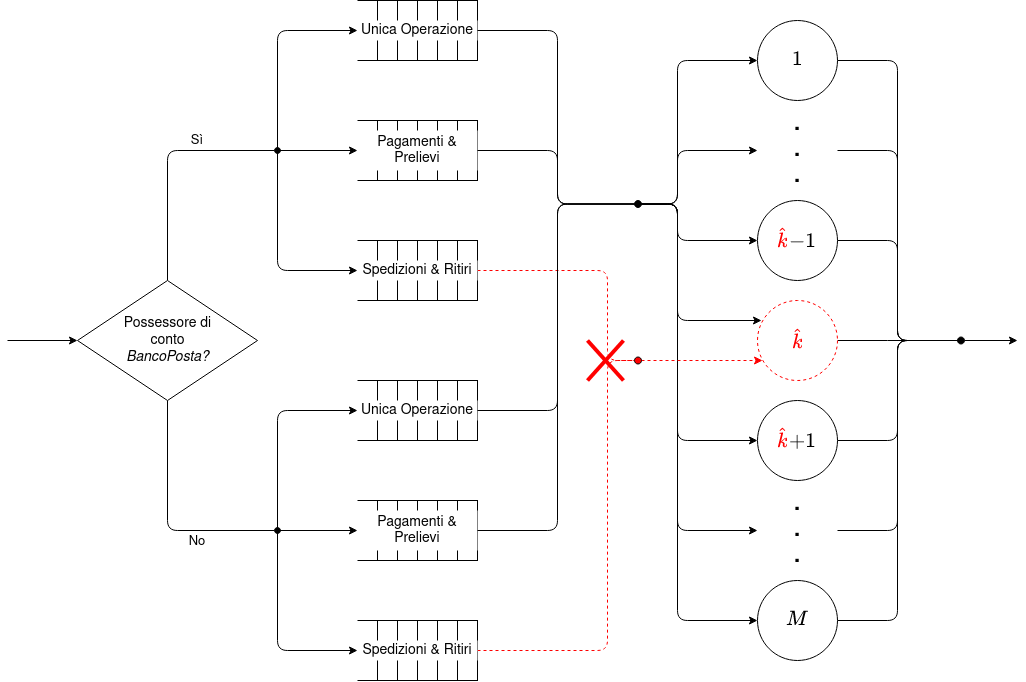
\includegraphics[width=0.5\linewidth]{modello-concettuale-sempl-1}
\caption{Blocco del flusso degli arrivi di tipo \sr{}}
\label{fig:validazione-semplificazione-1}
\end{figure}
Privando il sistema della generazione di arrivi di tipo \sr{}, come mostrato in figura \ref{fig:validazione-semplificazione-1} e fissando $M=3$, si ottengono i seguenti risultati:
\begin{itemize}
\item Mediante la simulazione:
\begin{itemize}
\item Un intervallo di confidenza al 95\% per il tempo medio d'attesa globale è pari a:
\begin{equation} 
\bar{d}_g = \sum_{i = 1}^4 p_{g,i}\cdot \bar{d}_{g,i} = (4.29 \pm 1.02)\ min
\end{equation}
\item Un intervallo di confidenza al 95\% per il tempo medio di risposta globale è pari a:
\begin{equation}
\bar{w}_g = \sum_{i = 1}^4 p_{g,i}\cdot \bar{w}_{g,i} = (14.56 \pm 1.29)\ min
\end{equation}
\end{itemize}

\item Mediante l'analisi effettuata in riferimento al modello a code riportato in figura \ref{fig:validazione-modello-analitico-1a}:
\begin{itemize}
\item Il tempo medio d'attesa globale ottenuto è pari a:
\begin{equation}
E[T_{Q_g}]^{KP} = 9.256825\ min 
\end{equation}
\item Il tempo medio di risposta globale ottenuto è pari a:
\begin{equation}
E[T_{S_g}] = 12.756807\ min 
\end{equation}
\end{itemize}
in accordo rispettivamente alle equazioni \ref{eqn:validazione-11} e \ref{eqn:validazione-13}.
\end{itemize}

I risultati ottenuti sono ragionevoli poiché:
\begin{itemize}
\item Il tempo d'attesa medio di un multiserver, a parità di utilizzazione, è teoricamente inferiore a quello di un single server a capacità equivalente, per via del fatto che $P_Q \leq \rho$.
\item Il tempo di risposta medio di un multiserver è asintoticamente equivalente a quello di un single server avente la medesima capacità nel caso in cui $\rho\to 1$. In questo caso, poiché:
\begin{itemize}
\item Un intervallo di confidenza al 95\% per l'occupazione media ottenuta tramite la simulazione è pari a:
\begin{equation}
\bar{x}_g = 0.70 \pm 0.03
\end{equation}
\item L'occupazione media teorica, in accordo alla \ref{eqn:validazione-8}, è pari a:
\begin{equation}
\rho_g = 0.725638
\end{equation}
\end{itemize}
le prestazioni del multiserver, in termini di risposta, sono inferiori al sistema a capacità concentrata.
\end{itemize}

È opportuno osservare che i risultati ottenuti in fase di simulazione sono stati computati mantenendo i tassi di servizio delle differenti tipologie di ticket, così come definiti nel modello delle specifiche (cap. \ref{chp:modello-specifiche}). Questo è ragionevole perché la media pesata dei differenti tassi di servizio è pari a quello definito nella \ref{eqn:validazione-6}.


\section{Blocco del flusso degli arrivi di tipo \uo{} e \pp{}}\label{sec:validazione-blocco-uo-pp}
Privando il sistema della generazione di arrivi di tipo \uo{} e \pp{}, come mostrato in figura \ref{fig:validazione-semplificazione-2}, si ottengono i seguenti risultati:
\begin{itemize}
\item Mediante la simulazione:
\begin{itemize}
\item Un intervallo di confidenza al 95\% per il tempo medio d'attesa globale ottenuto è pari a:
\begin{equation} 
\bar{d}_d = p_{d,1}\cdot \bar{d}_{d,1} + p_{d,2}\cdot \bar{d}_{d,2} = (6.04 \pm 1.88)\ min
\end{equation}
\item Un intervallo di confidenza al 95\% per il tempo medio di risposta globale ottenuto è pari a:
\begin{equation}
\bar{w}_d = p_{d,1}\cdot \bar{w}_{d,1} + p_{d,2}\cdot \bar{w}_{d,2} = (16.45 \pm 2.64)\ min
\end{equation}
\end{itemize}

\item Mediante l'analisi effettuata in riferimento al modello a code riportato in figura \ref{fig:validazione-modello-analitico-1b}:
\begin{itemize}
\item Il tempo medio d'attesa globale ottenuto è pari a:
\begin{equation}
E[T_{Q_d}]^{KP} = 5.769637\ min 
\end{equation}
\item Il tempo medio di risposta globale ottenuto è pari a:
\begin{equation}
E[T_{S_d}] = 15.769637\ min 
\end{equation}
\end{itemize}
in accordo rispettivamente alle equazioni \ref{eqn:validazione-24} e \ref{eqn:validazione-26}.
\end{itemize}

Poiché i valori teorici ricadono all'interno dei rispettivi intervalli, con un livello di confidenza del 95\%, il comportamento del simulatore è conforme al modello analitico \ref{fig:validazione-modello-analitico-1b}.

\begin{figure}[ht]
\centering
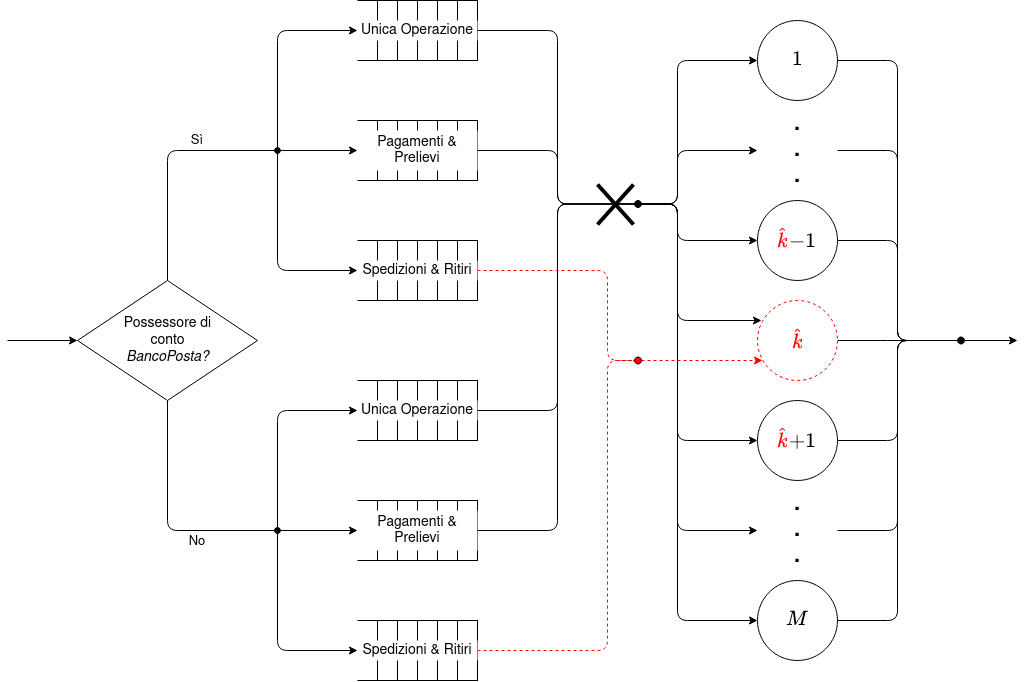
\includegraphics[width=0.5\linewidth]{modello-concettuale-sempl-2}
\caption{Blocco del flusso degli arrivi di tipo \uo{} e \pp{}}
\label{fig:validazione-semplificazione-2}
\end{figure}
